\section{Results}\label{sec:results}

\subsection{Admission Results}\label{sec:recall}

SDA exceeds each model's importance report and 1--10 importance rating in all 18 model--budget comparisons on the statedness-balanced pool (Figure~\ref{fig:results}). Qwen3-8B answer accuracy at $k=2$ rises from 43.0\% to 53.7\%. The rating is its strongest untrained policy on this pool; SDA exceeds it by 5.2 points at $k=2$.

\begin{table}[!htbp]
\centering
\caption{Admission policies on the statedness-balanced pool, Qwen3-8B; answer accuracy (\%). Criteria: 1--10 importance rating \citep{park2023generative}; ConsistencyGate \citep{consistencygate2026} (sampled and single-pass forms); A-MAC utility \citep{amac2026}; prediction error \citep{nemori2026} (candidate surprisal under the passage). App.~\ref{app:publishedbaselines} details published criteria.}
\label{tab:balancedbaselines}
\small
\setlength{\tabcolsep}{3pt}
\begin{tabular}{lccc}
\toprule
Admission policy & $k=1$ & $k=2$ & $k=3$ \\
\midrule
\multicolumn{4}{l}{\emph{Importance judgments of the untrained model}} \\
Importance report & 30.6 & 43.0 & 45.5 \\
1--10 importance rating & 35.8 & 48.5 & 50.7 \\
Implied-content wording & 31.7 & 44.9 & 47.7 \\
Statedness-cued wording & 31.4 & 42.7 & 45.5 \\
\addlinespace
\multicolumn{4}{l}{\emph{Admission criteria from published methods}} \\
ConsistencyGate, sampled & 24.0 & 35.0 & 40.8 \\
ConsistencyGate, single pass & 24.5 & 35.0 & 42.4 \\
A-MAC utility & 30.0 & 39.7 & 44.9 \\
Prediction error & 16.5 & 25.9 & 30.3 \\
\addlinespace
\multicolumn{4}{l}{\emph{Statedness rules}} \\
Reversed importance report & 23.7 & 29.8 & 33.1 \\
Unstated-first & 28.6 & 32.0 & 36.4 \\
Unstated-first with report ordering & 36.9 & 39.1 & 39.9 \\
\midrule
\textbf{SDA} & \textbf{40.5} & \textbf{53.7} & \textbf{51.8} \\
\addlinespace
\refrow Gold-concept selection & 47.4 & 54.3 & 51.5 \\
\bottomrule
\end{tabular}
\end{table}


Qwen3-8B SDA exceeds every baseline at every budget, reaching 40.5\%, 53.7\% and 51.8\% at $k=1,2,3$ (Table~\ref{tab:balancedbaselines}). At $k=2$, margins are 9.1 points over implied-content wording and 14.6 over unstated-first with report ordering, which exploits the original pool's composition (Table~\ref{tab:balancedpaired}). Published criteria implemented from their papers (App.~\ref{app:publishedbaselines}) fall below the untrained importance report: SDA exceeds each ConsistencyGate form by 18.7 points, A-MAC utility by 14.1 and Nemori's prediction error by 27.8 at $k=2$. The smallest margin is 6.9 points over A-MAC utility at $k=3$.

SDA increases useful-concept retention in both statedness conditions. For Qwen3-8B at $k=2$, the importance report retains the useful concept in 47.4\% of stated-concept and 31.2\% of unstated-concept episodes; SDA reaches 77.5\% and 63.4\%. Across the 173 unstated-concept episodes, answer accuracy gains over the importance report are 12.5, 9.6 and 9.6 points at $k=1,2,3$.

SDA exceeds each model's importance report in all 18 model--budget comparisons on the original pool, averaging 9.6 points at $k=2$ (Table~\ref{tab:sdabudget}). Qwen3-8B also exceeds its importance report on each development set and the held-out set (Table~\ref{tab:sdamain}). Closed-book and full-context readers reach 22.9\% and 63.9\%, bracketing SDA's 50.0\% on the original pool.

\begin{figure*}[t]
\centering
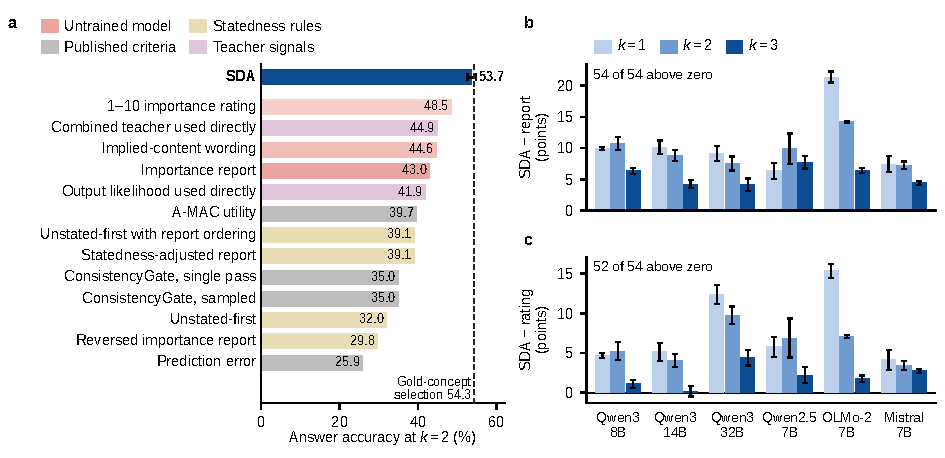
\includegraphics[width=\textwidth]{figures/fig_results.pdf}
\caption{SDA's answer accuracy gains (points) over (a) each model's importance report and (b) its 1--10 importance rating, across six models and budgets $k=1,2,3$ on the statedness-balanced pool.}
\label{fig:results}
\end{figure*}

\subsection{Robustness Across Candidate Pools}\label{sec:budgets}

The naming-balanced pool balances the naming cue left imbalanced by the statedness-balanced pool: four candidates are named per episode using five sentence templates at varying positions, and named candidates are useful 12.5\% of the time against a 12.6\% base rate. The pool with unstated distractors adds four confusable unstated concepts from the useful concept's semantic category to the original pool. The enlarged pool adds further concepts from other episodes, averaging 12.41 candidates.

SDA exceeds the importance report for every model at $k=2$ on all four pools in Figure~\ref{fig:apppools}. Across budgets, it exceeds the importance report in all 18 model--budget comparisons on the pool with unstated distractors and original pool, and 17 of 18 on the naming-balanced pool; the remaining comparison differs by 0.1 points (Table~\ref{tab:stress}, Table~\ref{tab:sdabudget}, Table~\ref{tab:namingrecall}). Qwen3-8B gains 11.0 points at $k=2$ on the enlarged pool (Table~\ref{tab:paired}) and improves within-episode ranking and useful-concept retention on the naming-balanced pool (Table~\ref{tab:namingbalanced}).

\begin{figure}[t]
\centering
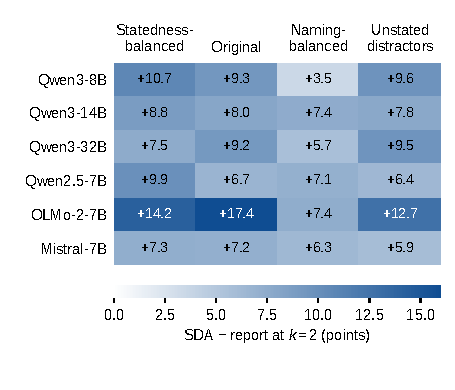
\includegraphics[width=\columnwidth]{figures/figS_pools.pdf}
\caption{Cells show SDA minus the importance report in answer accuracy points across candidate pools and models at $k=2$ stored concepts.}
\label{fig:apppools}
\end{figure}

\begin{figure*}[t]
\centering
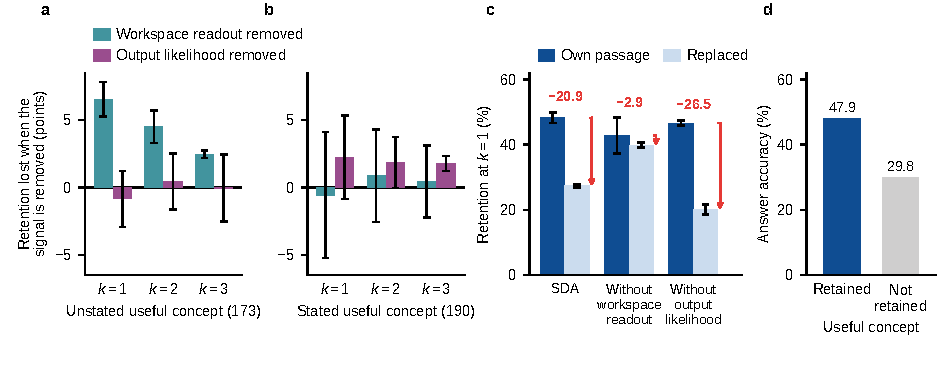
\includegraphics[width=\textwidth]{figures/fig_mechanism.pdf}
\caption{Teacher-signal removal and passage replacement affect useful-concept retention. (a,b) Statedness-balanced pool: SDA minus ablated students (points), averaging five models, $k=1,2,3$. (c) Qwen3-8B, original pool, $k=1$: retention (\%). (d) Frozen reader accuracy (\%) with versus without useful-concept retention, pooling unstated-concept episodes across SDA and the students trained without the workspace readout, using (a,b)'s models and budgets.}
\label{fig:mechanism}
\end{figure*}

\subsection{Ablations}\label{sec:ablations}\label{sec:scale}

The workspace readout supports retention of unstated useful concepts. Teacher-signal ablations train the same adapter after removing the workspace readout or output likelihood, fixing training episodes and step budget. On the statedness-balanced pool, removing the workspace readout lowers unstated useful-concept retention by 6.6, 4.5 and 2.5 points at $k=1,2,3$, in all five models at every budget: Qwen3-8B, Qwen3-14B, Qwen3-32B, Qwen2.5-7B and OLMo-2-7B. Removing output likelihood changes it by at most 0.8 points and lowers stated useful-concept retention by 2.2, 1.9 and 1.8 points at $k=1,2,3$ (Figure~\ref{fig:mechanism}a,b; Table~\ref{tab:teacherretention}). Across all episodes, removing output likelihood lowers answer accuracy by 1.6 and 1.7 points at $k=1,2$; removing the workspace readout lowers it by 0.7, 0.6 and 0.3 at $k=1,2,3$ (Table~\ref{tab:teacherretention}; per-model accuracy in Table~\ref{tab:teachermodels}).

Retaining the useful concept supports answer accuracy. Pooling unstated-concept episodes for SDA and students without the workspace readout across five models, three training runs and three budgets, the frozen reader answers 47.9\% correctly with the useful concept in memory and 29.8\% without it (Figure~\ref{fig:mechanism}d). Replacing it with SDA's next-ranked candidate on the 249 episodes where SDA retains it lowers Qwen3-8B answer accuracy from 54.6\% to 37.8\%, a paired decrease of 16.9 points, losing 59 answers and gaining 17.

Both ablations lower mean answer accuracy at every budget on the paired-passage set. Paired test-set episodes share candidates in different orders while retaining their passages, questions and useful concepts; the partner's useful concept is negative, so only the passage identifies usefulness (App.~\ref{app:pools}). Across 181 pairs, five models and 1,810 observations per budget, removing the workspace readout lowers useful-concept retention by 7.3 points and answer accuracy by 1.9 at $k=1$; removing output likelihood lowers answer accuracy by 1.3. Removing the workspace readout lowers retention at every budget (Table~\ref{tab:crosspairpooled}).

Passage replacement reveals dependence on the passage by substituting another episode's passage with candidates, labels and question fixed. On 363 original-pool episodes at $k=1$, Qwen3-8B SDA useful-concept retention falls by 20.9 points; the student without output likelihood loses 26.5 points, and the student without the workspace readout loses only 2.9 points, so its selections barely depend on the passage (Figure~\ref{fig:mechanism}c).

Distillation improves admission beyond direct teacher rankings. For Qwen3-8B on the statedness-balanced pool at $k=2$, the combined teacher used directly reaches 44.9\% answer accuracy, 8.8 points below SDA; output likelihood used directly is 11.8 points below (Table~\ref{tab:balanceddirect}, Table~\ref{tab:balancedpaired}). SDA trained through implied-content wording exceeds that wording at every budget (Table~\ref{tab:wordingdistill}). SDA changes how the model reports importance, not what its workspace readout encodes: at every tested Qwen3 scale, SDA raises pooled AUC on the development sets while the adapter-enabled model's workspace readout AUC changes by at most 0.0046 (Table~\ref{tab:sdascale}).

\subsection{Deployment}\label{sec:deployment}

SDA serves 242 candidates per second at 4.1\,ms per candidate through vLLM on one A100-80GB, against 290 at 3.4\,ms for the importance report, using prefix caching over 1,607 original-pool candidates after warm-up. Served Qwen3-8B answer accuracy is 50.1\%, within 0.3 points of the reference run's offline selections; top-2 memories agree on 91.7\% of episodes (App.~\ref{app:timing}). Enabling the adapter on every token changes four capability scores by at most 0.3 points (App.~\ref{app:capability}).
